\label{texfile:TemplateMesh}
A template mesh is a 2D finite-element mesh that is used, ultimately, for generating \mfus\ finite-difference meshes composed of cells.  As an intermediate step, a finite-element mesh is created, which is then used to define the \mf\ finite-difference cells.  Below is an example 
\footnote{See \tecplot\ layout file \texttt{MUT\_Examples$\backslash$6\_Abdul\_Prism\_Cell$\backslash$FIG Template Abdul.lay}. }
  showing an exploded view of a template mesh (bottom image) that was used as a basis for generating intermediate finite-element meshs for the GWF (middle image) and SWF (upper image) domains:
    \vspace{.2in} \\
    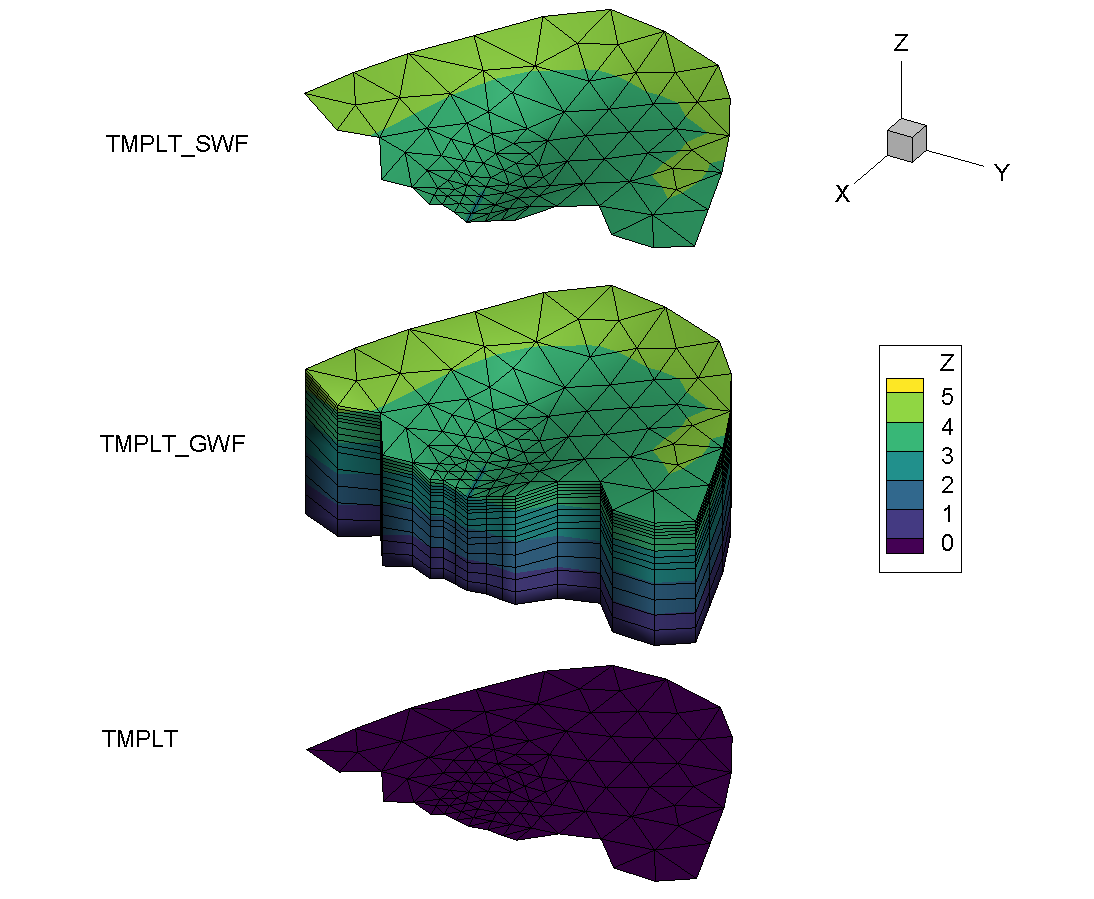
\includegraphics[width=0.9\textwidth]{tmpltAbdul}
    \vspace{.2in} \\
Note the following:
\begin{itemize}
  \item The template mesh is assigned an elevation of zero, and only the $xy$ coordinate data are used to define the other domains.
  \item The GWF domain has been assigned a base elevation of zero, and a variable top elevation. 
  \item The SWF domain has been assigned the same elevation as the GWF domain i.e.\ they are coincident.
\end{itemize} 

%\begin{figure}
%    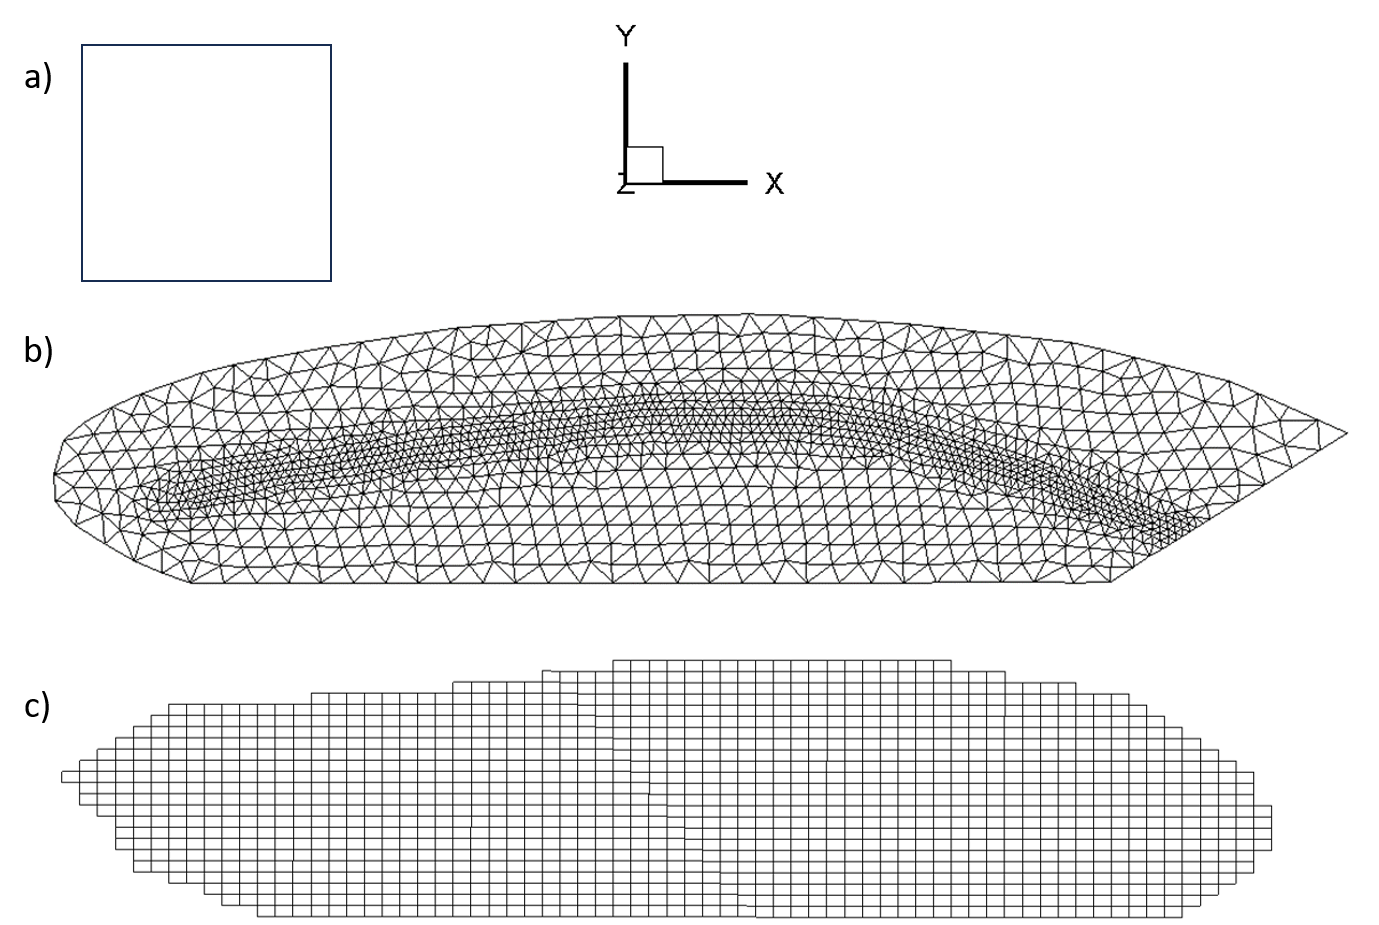
\includegraphics[width=\textwidth]{TemplateMeshes}
%    \caption{Sample template meshes a) a single rectangular element, b) an unstructured triangular-element mesh, and  c) an unstructured rectangular-element mesh}
%    \label{fig:Template Meshes}
%\end{figure}

 There are options for defining the template meshes:
\begin{description}
  \item[generate uniform rectangles] The file
  \item[2d mesh from gb] The value is assigned to all nodes in the top sheet of the TECPLOT\_GWF mesh.
  \item[2d quadtree mesh from groundwater vistas] The file
\end{description}
2d mesh from gb'
'
generate uniform rectangles'



In our example, the template mesh is defined by the following lines in the input file:
\begin{verbatim}
    generate uniform rectangles
    1.0, 1   !  Mesh length in X-direction and number of rectangular elements
    1.0, 1   !  Mesh length in Y-direction and number of rectangular elements
\end{verbatim}

The \texttt{generate uniform rectangles} instruction reads two lines of input data:
    \begin{enumerate}
        \item\textbf{xl, nbx}  Domain length and number of rectangles in the $x$-direction
        \item\textbf{yl, nby}  Domain length and number of rectangles in the $y$-direction
    \end{enumerate}
This data is used to generate a grid for a rectangular domain made up of uniform rectangles, which is
formed by subdividing the domain in the $x$-direction into \textbf{nbx} blocks, each of length \textbf{xl/nbx}.
The domain is subdivided in a similar fashion in the $y$-direction, using the second line of input data.

In our example, this results  in a single rectangular element that is 1 by 1 m in size, as shown in Figure~\ref{fig:Template Meshes}(a).






